\begin{figure}[h!]
\begin{center}
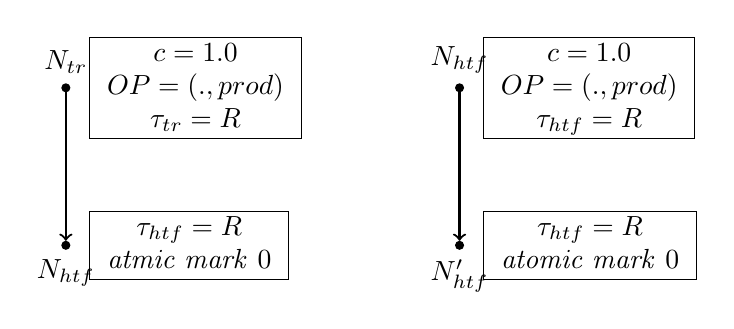
\begin{tikzpicture}[yscale=-1,
place/.style={circle,draw=black, fill=black, inner sep=0pt, 
              minimum size=1mm}]

\node[place] (1st) at (0, 0) [label=above: $N_{tr}$,
                              label=right: {
             \begin{tabular}{|c|}
               \hline
               $c=1.0$ \\
               $OP=(.,prod)$ \\
               $\tau_{tr}=R$ \\
               \hline
             \end{tabular} }] {};

\node[place] (2nd) at (0, 2) [label=below:  $N_{htf}$,
                                label=right: {
             \begin{tabular}{|c|}
               \hline
               $\tau_{htf}=R$\\
               \textit{atmic mark} $0$ \\
               \hline
             \end{tabular} }
] {};
        
	\draw[->, thick] (1st) -- (2nd);

\begin{scope}[xshift=5cm]
 \node[place] (1st) at (0, 0) [label=above: $N_{htf}$,
                              label=right: {
             \begin{tabular}{|c|}
               \hline
               $c=1.0$ \\
               $OP=(.,prod)$ \\
               $\tau_{htf}=R$ \\
               \hline
             \end{tabular} }] {};

\node[place] (2nd) at (0, 2) [label=below:  $N'_{htf}$,
                                label=right: {
             \begin{tabular}{|c|}
               \hline
               $\tau_{htf}=R$\\
               \textit{atomic mark} $0$\\
               \hline
             \end{tabular} }
] {};
        
	\draw[->, thick] (1st) -- (2nd);
\end{scope}

\end{tikzpicture}
\end{center}
\caption{Expansion of tr and htf}
\label{fig:ExpansionTrHtf}   
\end{figure}